We compare \sys\/ in HBase to the baseline HBase MemStore implementation.  
Our evaluation explores \sys's different policies and configuration parameters.  
We experiment with two types of production machines with directly attached SSD 
and HDD storage. 

We study HBase's throughput and latency under a variety of workloads. 
To reason about the results, we explore additional signals -- I/O statistics, 
GC metrics, etc.  

We present the experiment setup in Section~\ref{ssec:setup}, and the evaluation 
results in Section~\ref{ssec:results}. 

\subsection{Experiment Setup}
\label{ssec:setup}

Our experiments exploit two clusters with different hardware types. The first cluster consists of five 12-core Intel Xeon 5 
machines with 48GB RAM and 3TB SSD storage. The second cluster consists of five 8-core Intel Xeon E5620 servers 
with 24GB RAM and 1TB HDD storage. Both clusters have a 1Gbps Ethernet interconnect. We refer to these clusters as
SSD and HDD, respectively.

In each cluster, we use three nodes for HDFS and HBase instances, which share the hardware. The HDFS data 
replication ratio is 3x. HBase exploits two machines as region servers, and one as a master server. 

A region server runs  with 8GB heap, under G1GC memory management. 
We use the default memory layout,  which allocates $40\%$ of the heap (roughly 3GB) to the MemStore 
area, and $40\%$ more to the read-path block cache. We apply an asynchronous WAL in order to focus on real-time 
write-intensive workloads (a synchronous WAL implies an order-of-magnitude slower writes). The log aggregation
period is one second. 
%The number of worker threads is 8, number of disk-flush threads is 10, and the maximal number 
%of HFile's per store is 25. 

Data resides in one table, pre-split to fifty regions (i.e., each region server maintains twenty-five regions). 
The table has a single column family with four columns. 
%Our benchmarks build and query a dataset of 50-100 GB in each experiment. 

The workload is driven by the two remaining machines, each running up to 12 client threads. 
We use the popular YCSB benchmarking tool~\cite{Cooper:2010:BCS:1807128.1807152} to generate 
put and get requests. All puts write a full row (4 cells of 25 bytes each), and all gets retrieve
a single cell. Such small values are typical in production workloads~\cite{Wu2015}. 

In order to produce a high load, updates are batched on the client side in 10KB buffers. 
In each experiment, all operations draw keys from the same distribution over a key range
of 100M items. We experiment with two distributions: heavy-tailed (Zipf) and uniform (the latter 
is less representative of real workloads and is studied for reference only). The Zipf distribution 
is generated following the description in~\cite{Gray:1994:QGB:191839.191886}, with $\theta=0.99\%$ 
(YCSB standard).

Each experiment consists of 500M writes and possibly concurrent reads. 
Depending on the setting (workload, algorithm, and hardware type), 
the duration of 
a single experiment  varies from approximately 1.5 hours to over 12 hours.  

\subsection{Evaluation Results}
\label{ssec:results}

We compare the different \sys\/ policies (\basic, \eager, and \adp\/) to the legacy MemStore implementation, to which we refer as 
\none. Here, \adp\/ is studied under multiple 
redundancy thresholds: $R=0.2$, $R=0.35$ and $R=0.5$ (the smaller the ratio, the more aggressively
the policy triggers in-memory compaction).  

\sys's parameters  $A$ (active segment fraction bound) and $S$ (pipeline number of segments bound)  
are tuned to values that optimize performance for the \basic\ version of \sys. We use $A=0.02$ and $S=5$.
Section~\ref{ssec:tuning} presents our parameter exploration. 

\begin{figure*}[tb]

  \centering
  
  \begin{subfigure}[t]{1.1\columnwidth}
      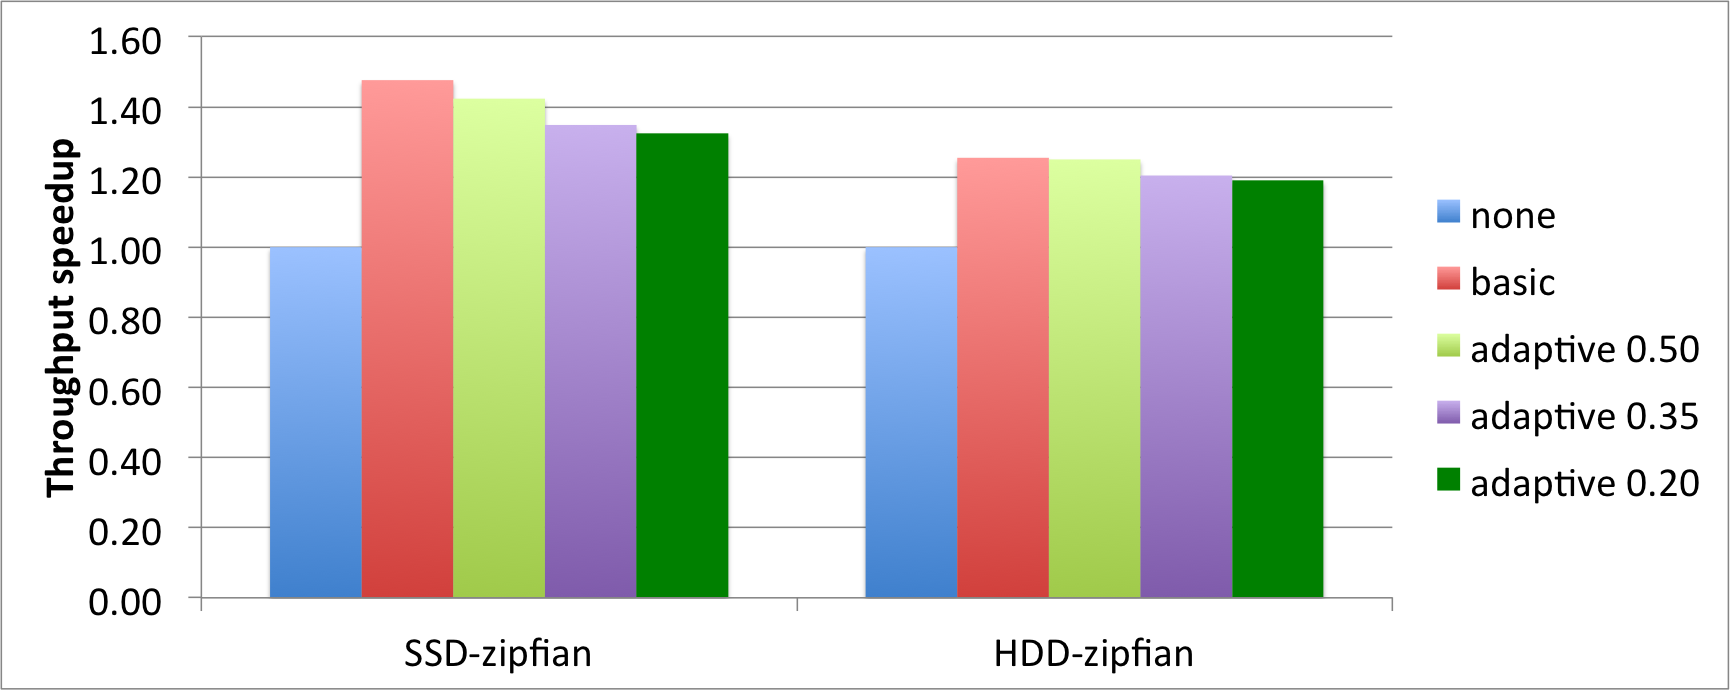
\includegraphics[width=\figw]{Figs/throughput-zipfian.png}
      \caption[]{Zipf distribution}
    \label{fig:write-throughput:zipf}  
  \end{subfigure}   \hskip .1\columnwidth
  \begin{subfigure}[t]{0.8\columnwidth}
      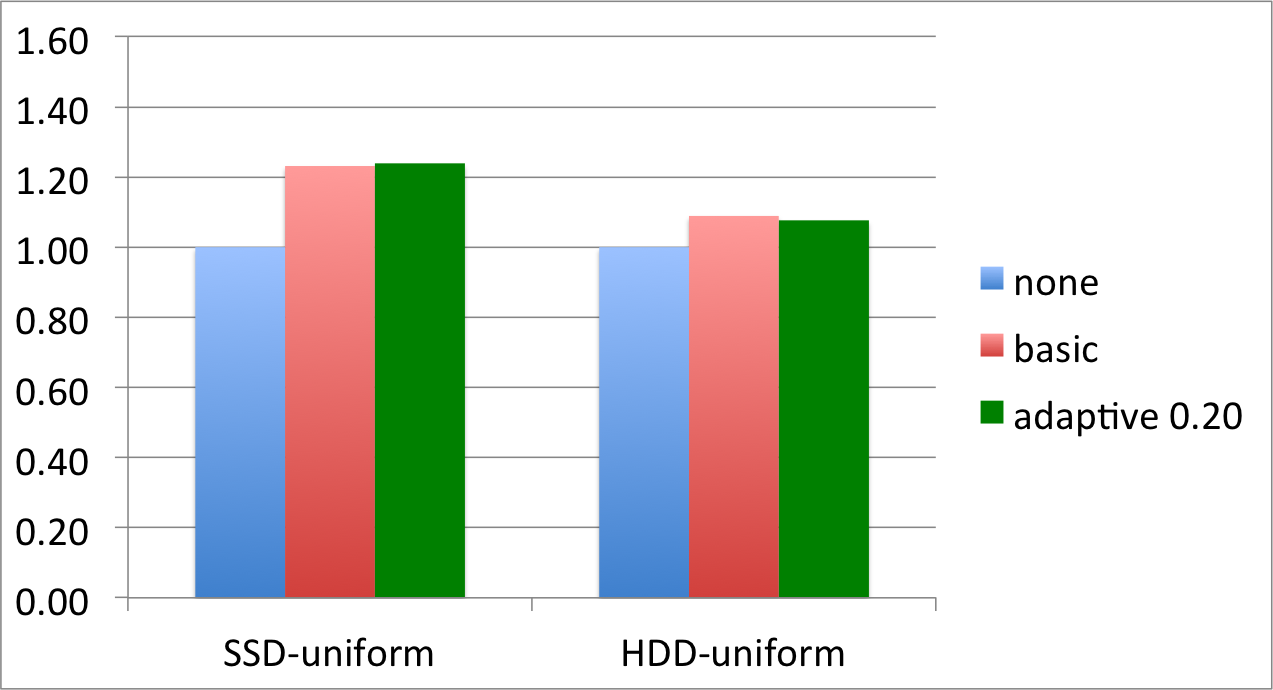
\includegraphics[width=\figw]{Figs/throughput-uniform.png}
      \caption[]{Uniform distribution}
    \label{fig:write-throughput:uniform}
  \end{subfigure}

\caption{Write throughput speedup vs \none\/ (HBase legacy MemStore) achieved by \sys\/ with \basic\/ and \adp\/ policies. 
Measured on the Zipf and uniform key distributions, on SSD and HDD hardware. In SSD systems, 
\basic\/ increases the write throughput by close to $48$\%. 
} 
\label{fig:write-throughput}
\end{figure*}

\begin{table*}
  \centering

        \begin{tabular}{|c|c|c|c|c|c|}
      \hline
       & Zipf, SSD & Zipf, HDD & Uniform, SSD & Uniform, HDD \\
      \hline
\none & $75{,}861$  & $60{,}457$ & $74{,}971$ & $35{,}342$ \\
\basic & $115{,}730$ & $78{,}392$ & $92{,}816$   & $38{,}488$ \\
      \hline
    \end{tabular}


\caption{Write throughput (operations per second) of the best \sys\/ policy (\basic\/) vs \none, across multiple key distributions and disk hardware types. }
\label{tab:write-throughput}
\end{table*}

\begin{table*}
  \centering
  
    \begin{tabular}{|c|c|c|c|c|}
      \hline
      Policy & $\#$flushes, SSD & $\#$compactions, SSD & $\#$flushes, HDD & $\#$compactions, HDD\\
      \hline
      \none & 1468	&524&	1504 & 548 \\
\basic & 1224&	355&	 1210 & 443 \\
\adp\/ (R=0.5) &922&	309&	879 & 316 \\
\adp\/ (R=0.35) & 754&	261&	711 &248 \\
\adp\/ (R=0.2) & 631	&209	&630 &216 \\
%\eager\ & {\bf 695}	& {\bf 242} &	667 & 242 \\
      \hline
    \end{tabular}

  \caption{Number of flushes and compactions, measured for \none\/ vs \sys\/ policies, for the Zipf key distribution.  }
  \label{tab:counters}
\end{table*}

\begin{figure*}[t]
  \centering
  
  \begin{subfigure}[t]{\columnwidth}
      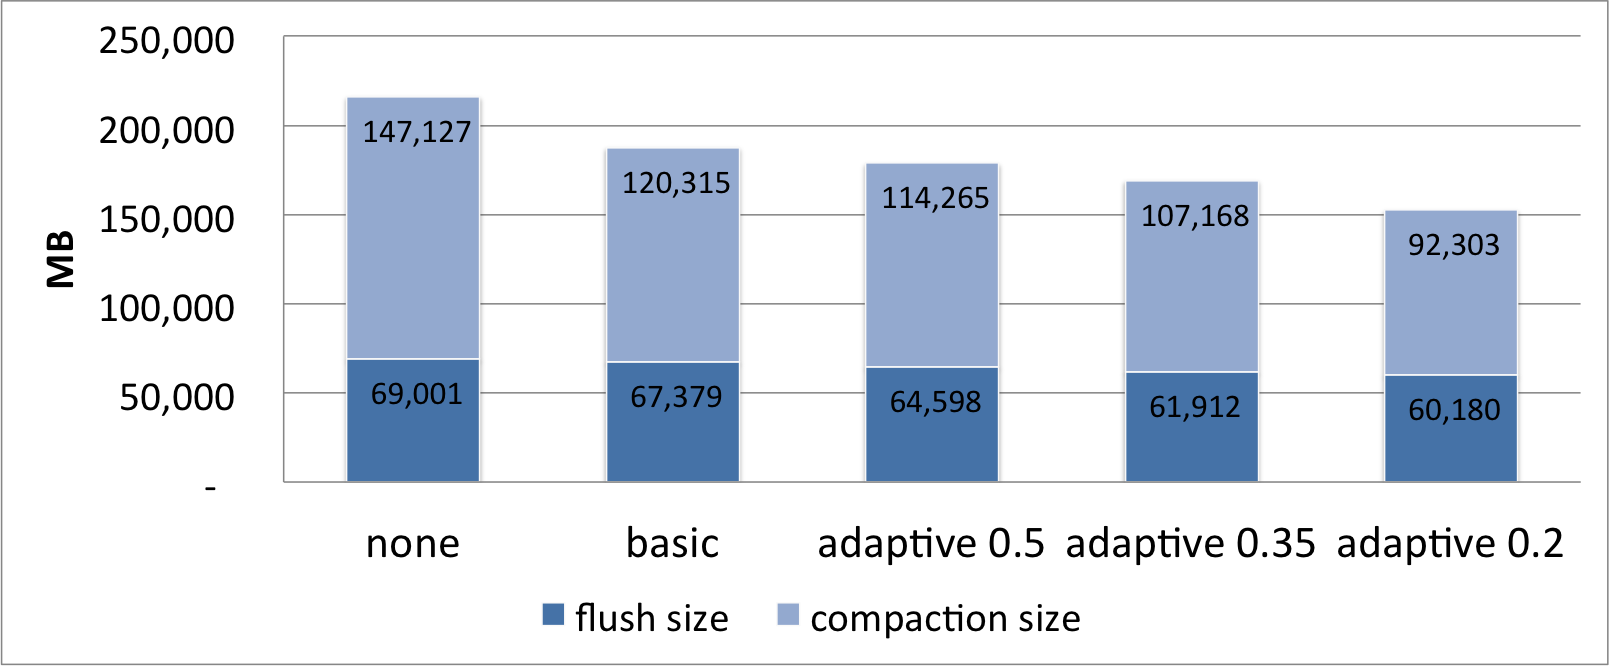
\includegraphics[width=\figw]{Figs/volume-ssd.png}
      \caption[]{SSD}
    \label{fig:volume:ssd}
  \end{subfigure}
  \begin{subfigure}[t]{\columnwidth}
      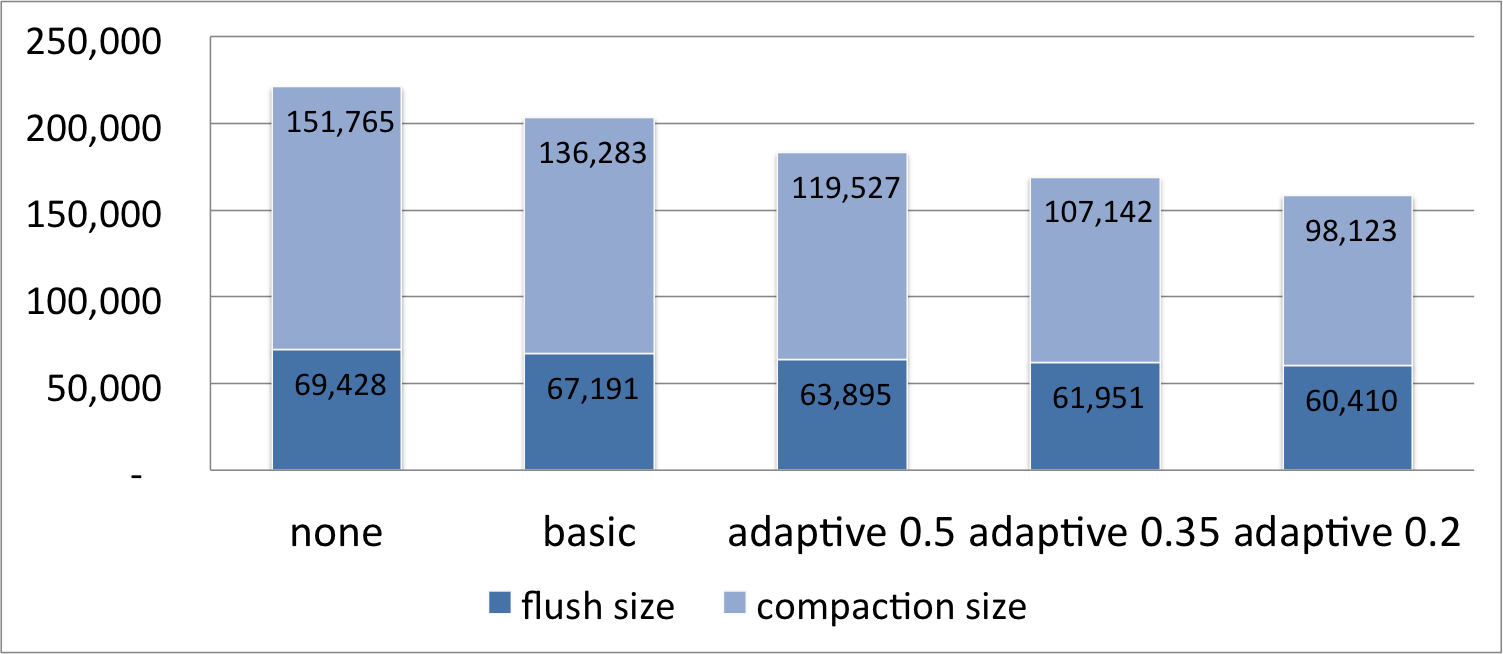
\includegraphics[width=\figw]{Figs/volume-hdd.png}
      \caption[]{HDD}
    \label{fig:volume:hdd}
  \end{subfigure}

  \caption{Bytes written by flushes and compactions, measured for \none\/ vs \sys\/ policies, for the Zipf key distribution. 
  The \adp\/ policy provides double-digit savings for disk I/O. }
  \label{fig:volume}
\end{figure*}

\subsubsection{Write-Only Workloads}

Our first benchmark set exercises only put operations. It starts from an empty table and performs 500M puts, 
in parallel from 12 client threads. We study the Zipf and  uniform key distributions. The experiments measure
write throughput (latency is not meaningful because puts are batched), as well as disk I/O and GC metrics. 
Every data point is the median among five runs. 

\paragraph{Write throughput} 
Figure~\ref{fig:write-throughput} depicts the performance speedup for
\none, \basic, and \adp. Table~\ref{tab:write-throughput} provides the absolute throughput numbers. 
For the Zipf benchmark, the maximal speedup is $47.6\%$ on SSD and $25.4\%$ on HDD. For the uniform benchmark, 
which has neither redundancy not locality, they are $23.8\%$ and $8.9\%$, respectively. 
The gain is significantly larger for the system with SSD storage, 
which is much faster on the I/O side. Being more CPU-bound than I/O-bound, its write throughput is more dependent on 
the MemStore speed than on background writes to the filesystem.  

Surprisingly, the \basic\/ policy, which flattens and merges segment indices but avoids 
redundancy elimination, yields the largest throughput gain. We explain this as follows. By reducing the active 
segment size to $A=2$\% of the MemStore size, all \sys\/ policies improve insertion time of new versions 
into the dynamic index through improved locality of access and search time in the skiplist. However, 
they affect the garbage collection in different ways. \basic\/ adds negligible overhead to 
garbage collection by recycling the index arrays. Similarly to \none, it releases memory in big bursts
upon disk flush. 

\eager\ is not included in this figure, because its performance with these parameters is below the baseline, as we show in the sequel.
It eliminates redundant data at a constant high rate,
which is less friendly for generational GC. And as we further show below, GC overhead is a strong predictor for 
overall 
performance. 

\adp\/ strikes a balance between \basic\/ and \eager. Its performance is much closer to \basic\/ 
because it is workload-driven and selective about the regions in which it performs in-memory compaction.  



Note that \adp\/ is only marginally slower than \basic\/ ($3$\% to $7$\% throughput for the Zipf 
distribution on SSD, immaterial in other cases).  In what follows, we substantiate  its savings 
on the I/O side. Going forward, we focus on the more realistic Zipf workload.
%, and  forgo the \eager\/ heuristic. 

\paragraph{I/O metrics}

\begin{figure}[htb]
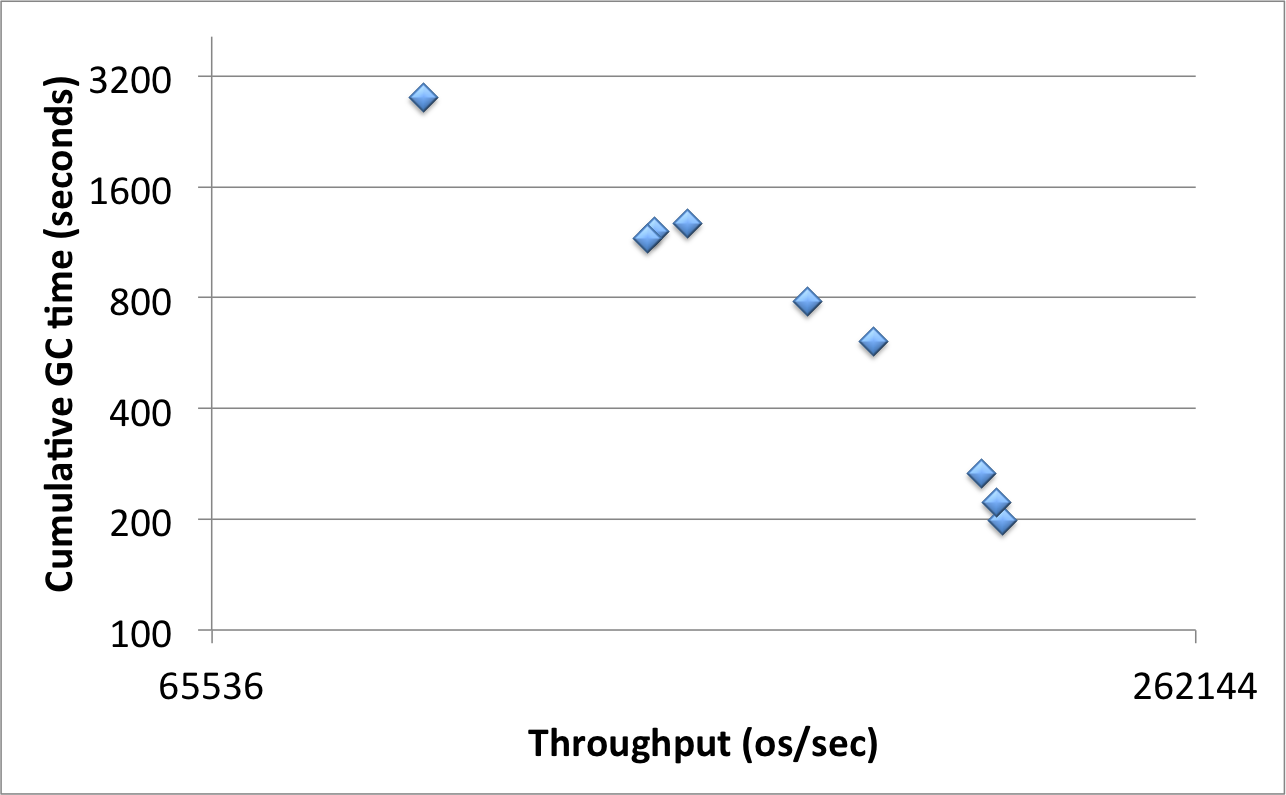
\includegraphics[width=\figw]{Figs/gc-throughput-log2.png}
\caption{GC time (cumulative, per minute) vs write throughput, measured on SSD machines 
for multiple \sys\/ policies and configurations, for the Zipf  key distribution. Each data point 
depicts the throughput vs GC time of one experiment. Both axes are in log-log scale.  
The graph shows a clear negative correlation between the two metrics. 
}
\label{fig:gc-throughput-log2}
\end{figure}

\begin{figure*}[t]
  \centering
  
  \begin{subfigure}[t]{.9\columnwidth}
      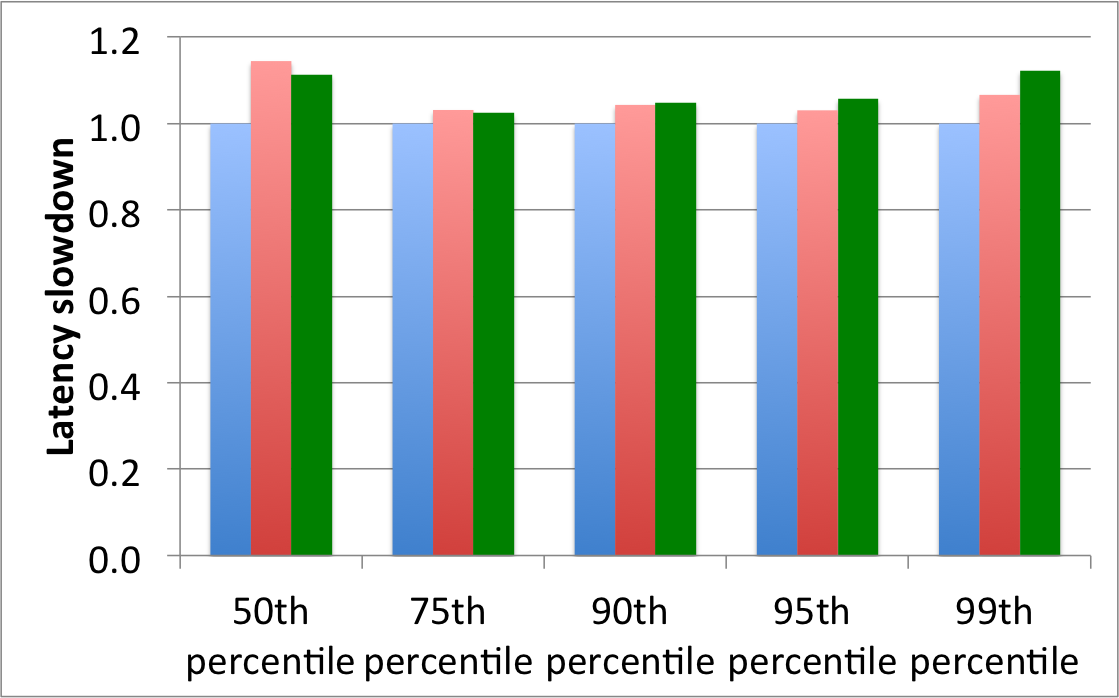
\includegraphics[width=\figw]{Figs/latency-ssd.png}
      \caption[]{SSD}
    \label{fig:latency:ssd}
  \end{subfigure}
  \begin{subfigure}[t]{1.1\columnwidth}
      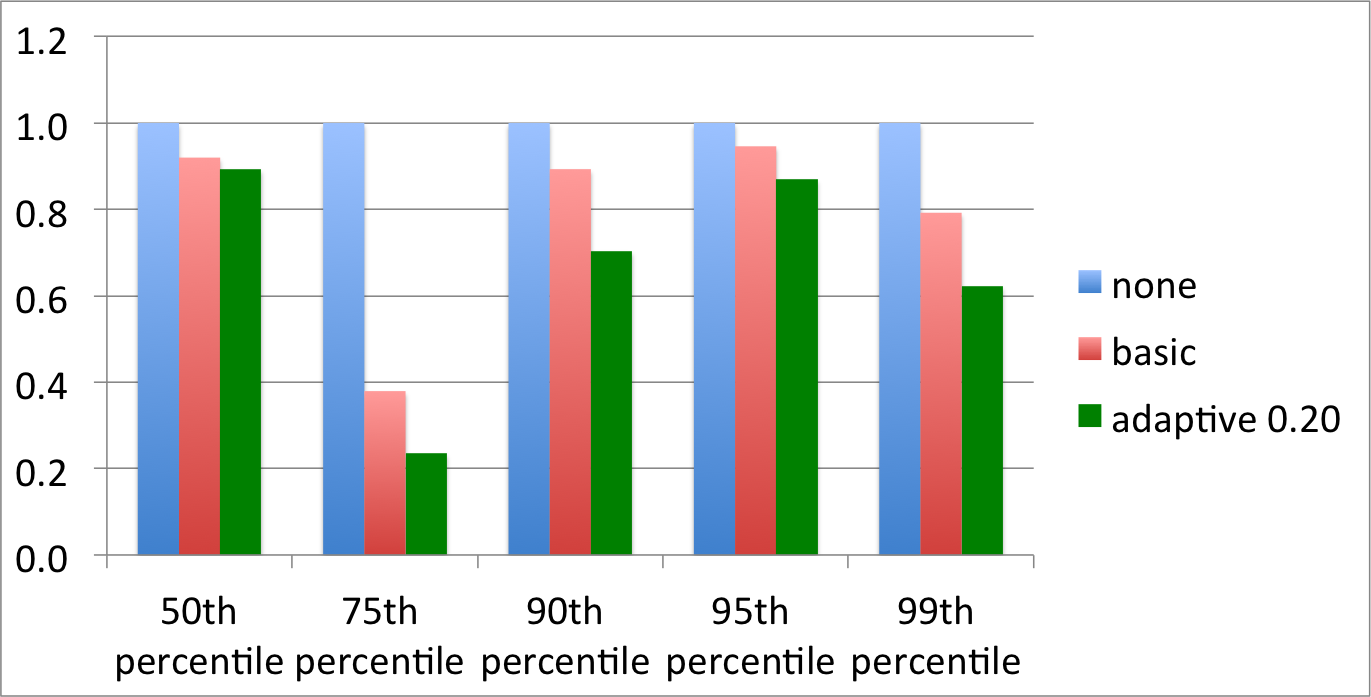
\includegraphics[width=\figw]{Figs/latency-hdd.png}
      \caption[]{HDD}
    \label{fig:latency:hdd}
  \end{subfigure}

  \caption{Read latency speedup (respectively, slowdown) of \basic\/ and \adp\/ versus \none, under high write contention.
  Latencies are broken down by percentile. In HDD systems, \adp\/ delivers up to $40$\% tail latency reduction. 
  }
  
  \label{fig:latency}
\end{figure*}

With respect to disk use by flushes and compactions, the picture is reversed. In this regard, 
\basic\/ provides modest savings. It writes $13$\% less bytes than \none\/ on SSD, and $8$\% 
on HDD. In contrast, \adp\ slashes the number of flushes and compactions by $58\%$ and $61$\%, 
respectively, and the number of bytes written by almost $30\%$. As expected, the lower the 
redundancy estimate threshold $R$, the more aggressive the algorithm, and consequently, 
the higher the savings. Figure~\ref{fig:volume} and Table~\ref{tab:counters} summarize the results. 

Note that the amount of data written to WAL %,186GB 
(approximately $45$\% of the write volume) remains constant across all  experiments. 
HBase operators often choose placing log files on inexpensive hard disks, since they are only needed for recovery,
and so disk wear is not a major concern for WAL data.

All-in-all, there is a tradeoff between the write throughput and storage utilization 
provided by the different \sys\/ policies. \adp\/ provides multiple operating points that trade major 
storage savings for minor performance losses.

\paragraph{Garbage collection}
 Redundancy elimination proved to be less impactful 
than memory management overhead, especially in systems with fast SSD hardware. 
Figure~\ref{fig:gc-throughput-log2}, which studies GC overhead for a range of policies and tuning 
parameters, further corroborates this hypothesis. It shows a clear negative correlation between the 
GC time and the write throughput. 
Note that this does not necessarily mean that GC time is the only reason for performance reduction. Rather,
GC cycles may be correlated with other costs, e.g., memory fragmentation, which reduces locality.

\anastas{
\paragraph{Basic Serialized Index}
We also experiment with the serialized segments where index is allocated on the mslab (Section~\ref{ssec:offheap}). We study the write-only workload as explained above with zipf key distribution and SSD hardware. The serialized segments are proposed for the case when both index and data are allocated on mslab. Figure~\ref{fig:write_only_off_heap} presents the throughput speedup over \none\/ for \basic\/ policy based on flat or serialized segments. In all benchmarks the data is allocated on on-heap or off-heap mslabs, while only for serialized \basic\/ also the index is allocated in the same mslab. For the flat \basic, the speedup is $27\%$ on-heap and $29\%$ off-heap. For the serialized \basic, the speedup is $33\%$ on-heap and $44\%$ off-heap. The gain from the serialized \basic\/ is larger for the off-heap case, because when index is taken off-heap even less work is left to JVM GC. 

\begin{figure}[htb]
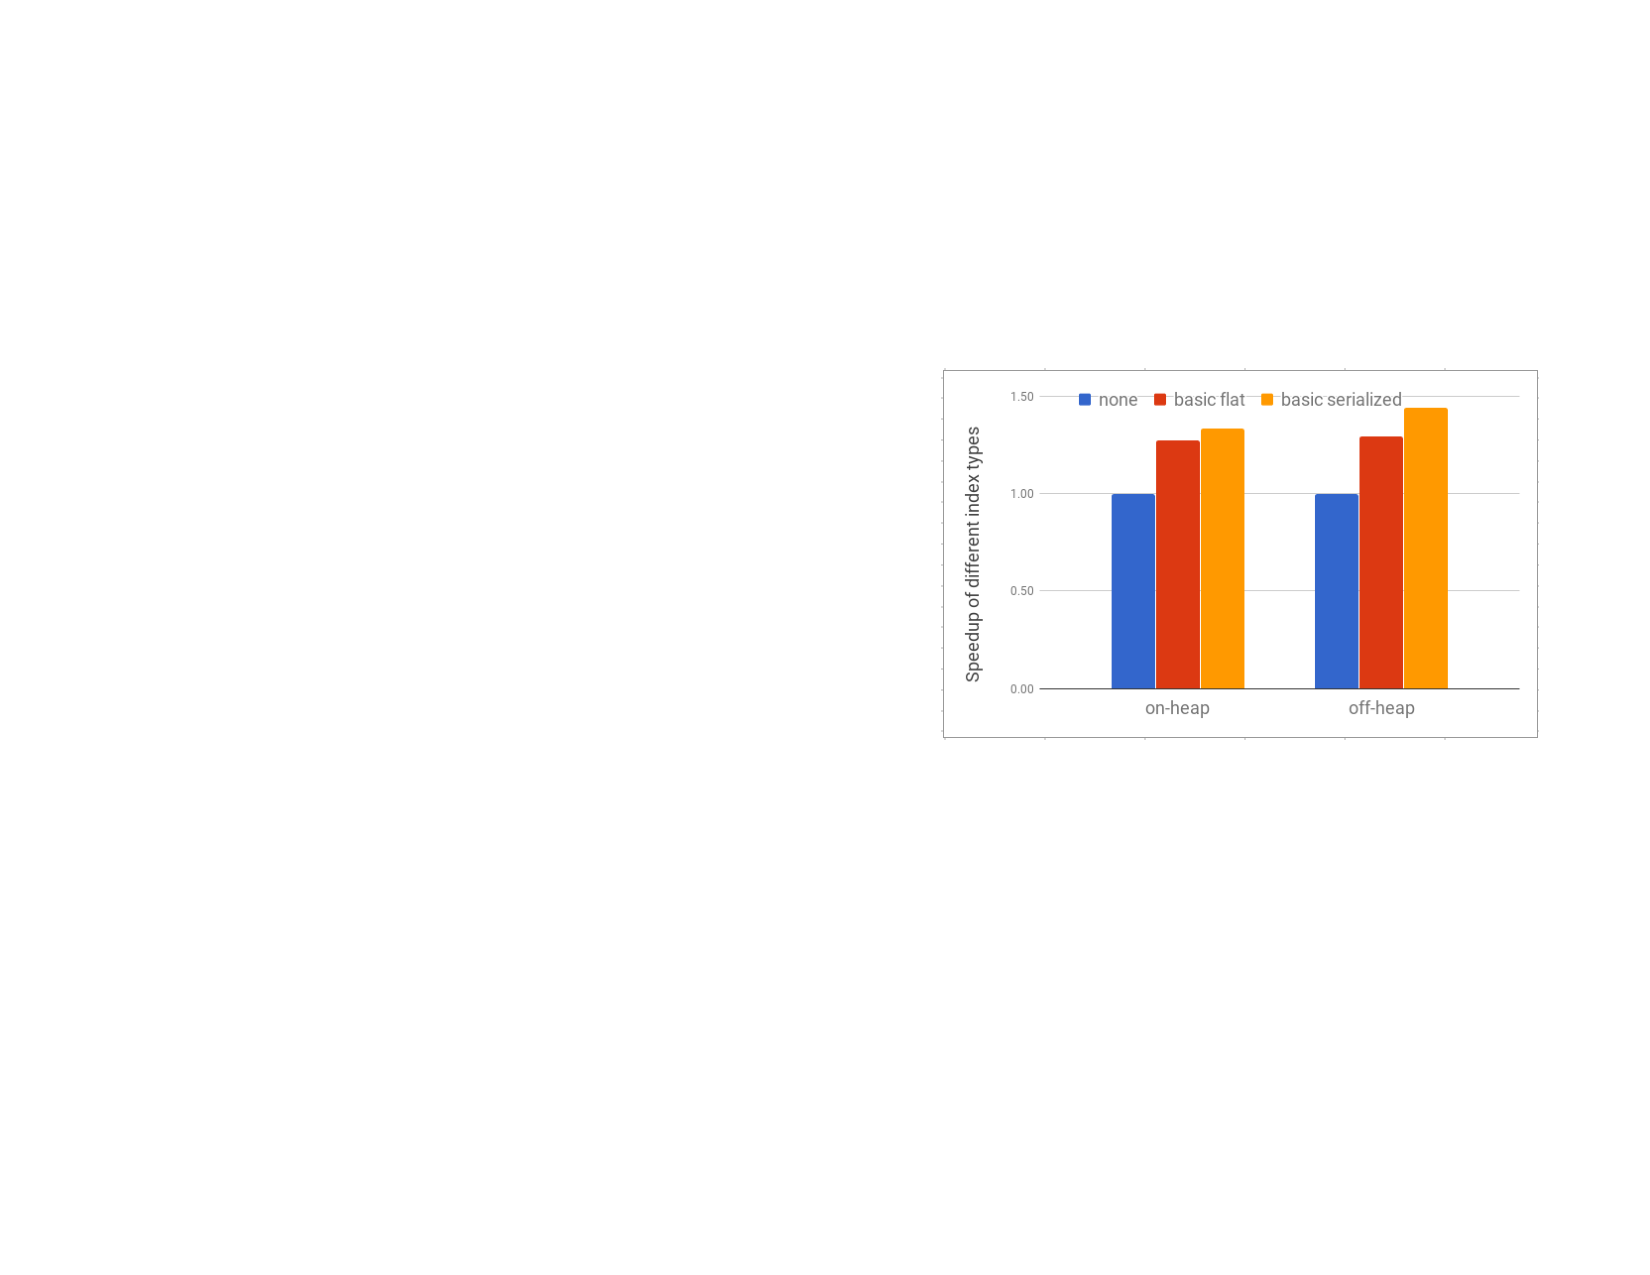
\includegraphics[width=\figw]{Figs/write-only-off-heap.pdf}
\caption{Throughput Speedup when using flat and serialized segments allocated on mslab (off-heap and on-heap).
}
\label{fig:write_only_off_heap}
\end{figure}
}

\subsubsection{Read-Write Workloads}

Our second benchmark studies read latencies under heavy write traffic. 
We run batched puts from 10 client threads and single-key gets from two other threads. 
The keys of all operations are distributed identically (Zipf). We measure the $50$th, 
$75$th, $90$th, $95$th and $99$th get latency percentiles. Figure~\ref{fig:latency} 
depicts the relative latency slowdown of \basic\/ and \adp\/ ($R=0.2$) versus \none.
%(values greater than 1 mean slowdown). 

The HDD systems enjoy a dramatic reduction in tail latencies ($15$\% to $40$\% for \adp). 
We explain this as follows. The tail latencies are cache misses that are served from disk. 
The latter are most painful with HDDs. Thanks to in-memory compaction, \adp\/ prolongs 
the lifetime of data in MemStore. Therefore, more results are served from MemStore, i.e., 
there are less attempts to read from cache, and consequently from disk, in case of a cache miss.  

In SSD systems, the get latencies are marginally slower in all percentiles (e.g., the 
$95$th percentile is $2.13$ms in \none\/ versus $2.26$ms in \adp). This happens
because most reads are dominated by in-memory search speed, which depends on the 
number of segments in the MemStore pipeline (in our experiment, 5). The other factor
is increased GC overhead in \adp\/ that stems from redundancy elimination. 


 \remove{ 


We compare the strategies by measuring their throughput and latency. In addition we measure the write volume, that is the number of KB written to the file system, and the cumulative GC time of each run.

The results of the following experiments are presented:
(1) demonstrating the insight from different sets of experiments showing that GC overhead is a great throughput predictor,
(2) write-only workload - comparing all 4 strategies,
(3) mixed read-write workload - showing reduction in read latencies of \basic\ and \magic\ strategies with respect to \none.
(4) evaluating different settings of the \basic\ strategy in order to find its optimal configuration,


\paragraph{Write-only workload.}
Each run creates an empty 50 regions table and then utilizes 12 threads to run 500 million update operations, each writing to all columns. Each such run is repeated 5 times. 
We measure total  throughput and total volume of MB written to files. We present here the performance results of the run with the median throughput among 5 runs.

Figures~\ref{fig:throughput-ssd} and~\ref{fig:throughput-hdd} depict the lift in throughput \basic, \magic, and \eager\ achieve over \none in SSD and HDD, respectively.
Tables~\ref{fig:counters:ssd} and ~\ref{fig:counters:hdd} present the number of flushes, disk compactions and WAL files generated during the experiment.
Figures~\ref{fig:volume-ssd} and~\ref{fig:volume-hdd} depict the write volume in every setting. 
\magic demonstrates the tradeoff between throughput and write volume. As we increase the compaction threshold more in-memory compaction are triggered which degrades the throughput but at the same time reduces the write volume.
At the extremes are \basic\ with the highest throughput and \eager with lowest write volume.
\basic\ and \magic\ both run with $2\%$ active segment. In SSD the limit on the size of the pipeline is 5 and in HDD it is 4.
\eager\ runs with $25\%$ active segments and limit of 2 on the size of the pipeline.
The uniques thresholds for \magic\ are $0.2$, $0.35$, and $0.5$.


\begin{table}[!t]
  \centering
  
  \begin{subfigure}[tb]{\columnwidth}
      \centering\small
    \begin{tabular}{|c|c|c|c|}
      \hline
      Policy & $\#$flushes & $\#$compactions & $\#$WAL files\\
      %\hline
      \hline
      \none & 1468	&524&	789 \\
\basic & 1224&	355&	806 \\
\adp\/ (R=0.5) &922&	309&	678 \\
\adp\/ (R=0.35) & 754&	261&	615 \\
\adp\/ (R=0.2) & 631	&209	&533 \\
\eager\ & 695	&242&	490 \\
      \hline
    \end{tabular}
	\caption[]{SSD}
    \label{fig:counters:ssd}
  \end{subfigure}
  
  \begin{subfigure}[t]{\columnwidth}
    \centering\small
    \begin{tabular}{|c|c|c|c|c|}
      \hline
        Policy & $\#$flushes & $\#$compactions & $\#$WAL files\\
      %\hline
      \hline
      \none & 1504 & 548 & 743 \\
\basic & 1210 & 443 & 808 \\
\adp\/ (R=0.5) & 879 & 316 & 695 \\
\adp\/ (R=0.35) & 711 & 248 & 650 \\
\adp\/ (R=0.2) & 630 & 216 & 556 \\
\eager\ & 667 & 242 & 536 \\
      \hline
    \end{tabular}
	\caption[]{HDD}
    \label{fig:counters:hdd}
  \end{subfigure}

  \caption{I/O metrics (flushes, compactions, and bytes written) measured for \none\/ vs \sys\/ policies, for the Zipf key distribution. 
  \sys\/ provides double-digit savings to disk I/O. The impact of I/O reduction is the largest for SSD hardware. }
  \label{fig:counters}
\end{table}

\begin{figure}[htb]
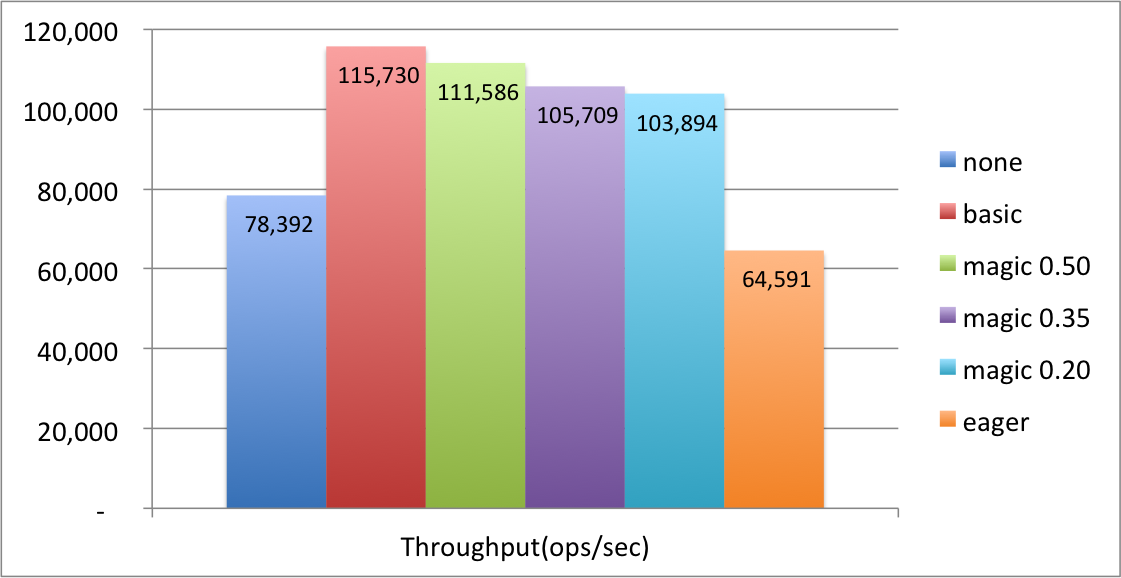
\includegraphics[width=\figw]{Figs/throughput-ssd.png}
\caption{{\bf  Throughput measured in SSD.} Zipf distribution.
}
\label{fig:throughput-ssd}
\end{figure}

\begin{figure}[htb]
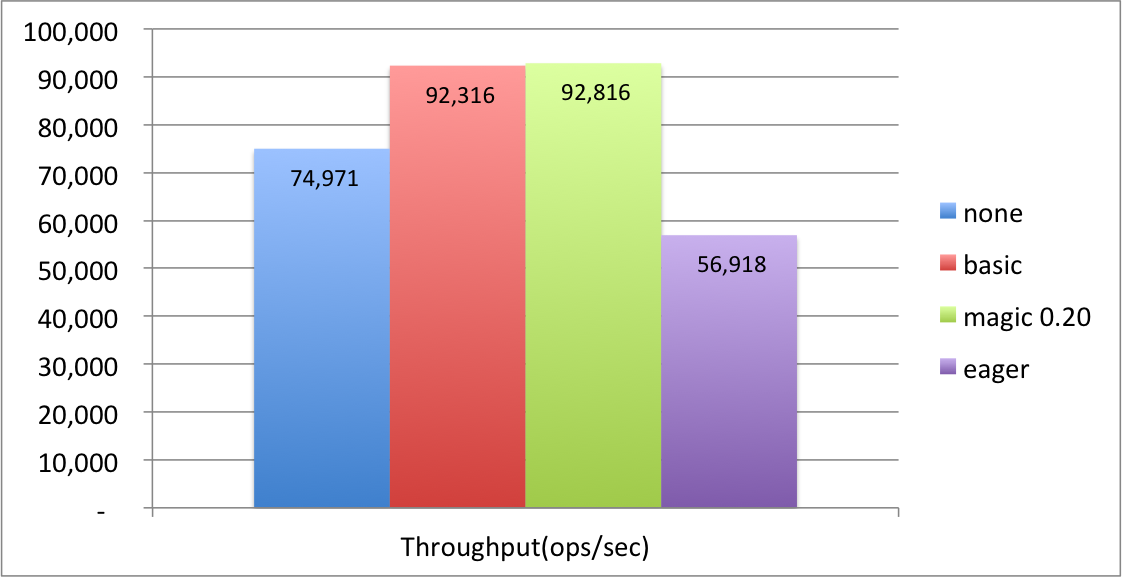
\includegraphics[width=\figw]{Figs/throughput-hdd.png}
\caption{{\bf  Throughput measured in HDD.} Zipf distribution. 
}
\label{fig:throughput-hdd}
\end{figure}




\begin{figure}[htb]
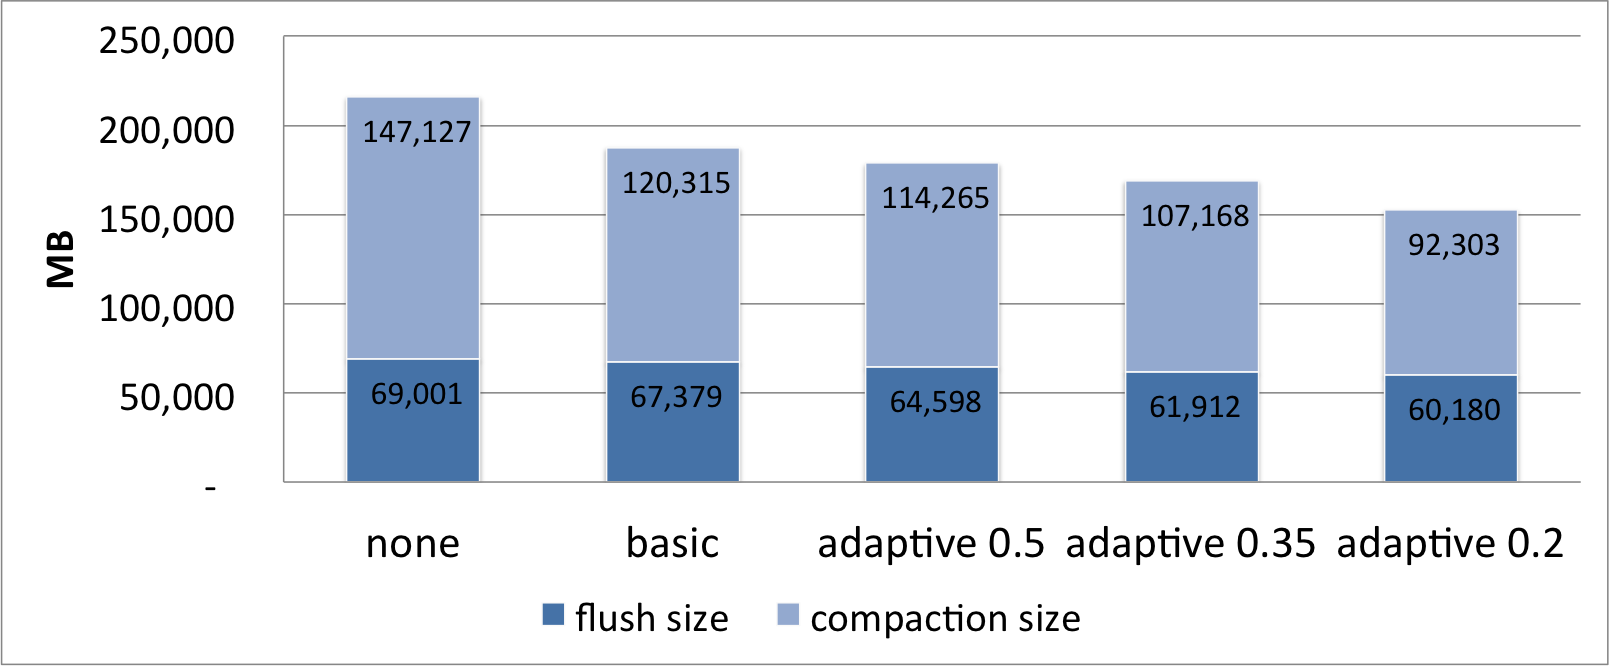
\includegraphics[width=\figw]{Figs/volume-ssd.png}
\caption{{\bf  Write volume in SSD.} Zipf distribution.
}
\label{fig:volume-ssd}
\end{figure}

\begin{figure}[htb]
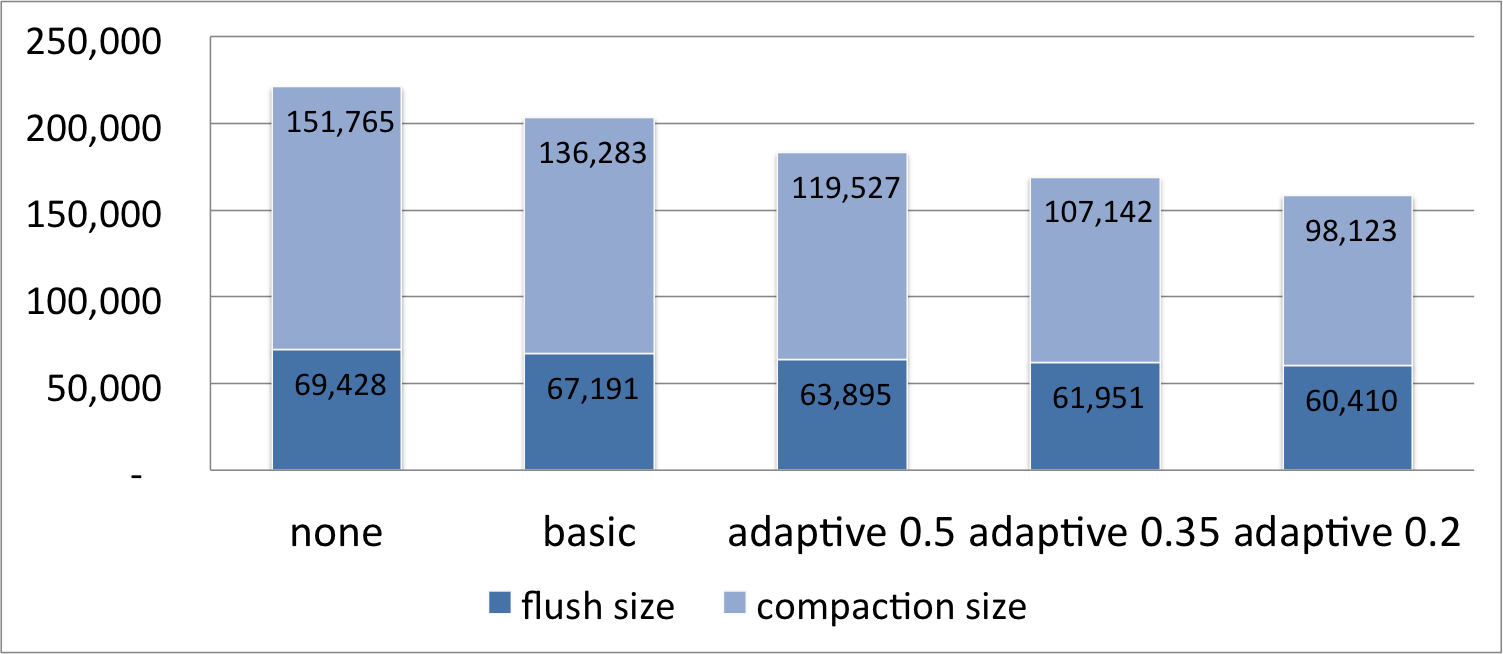
\includegraphics[width=\figw]{Figs/volume-hdd.png}
\caption{{\bf  Write volume in HDD.} Zipf distribution.
}
\label{fig:volume-hdd}
\end{figure}

Figures~\ref{fig:throughput-ssd-uniform} and~\ref{fig:throughput-hdd-uniform} depict the throughput results with uniform distribution in SSD and HDD, respectively.
Tables~\ref{fig:counters-uniform:ssd} and ~\ref{fig:counters-uniform:hdd} present the number of flushes, disk compactions and WAL files generated during the experiment.
Figures~\ref{fig:volume-ssd-uniform} and~\ref{fig:volume-hdd-uniform} depict the write volume in every setting. 


\begin{figure}[htb]
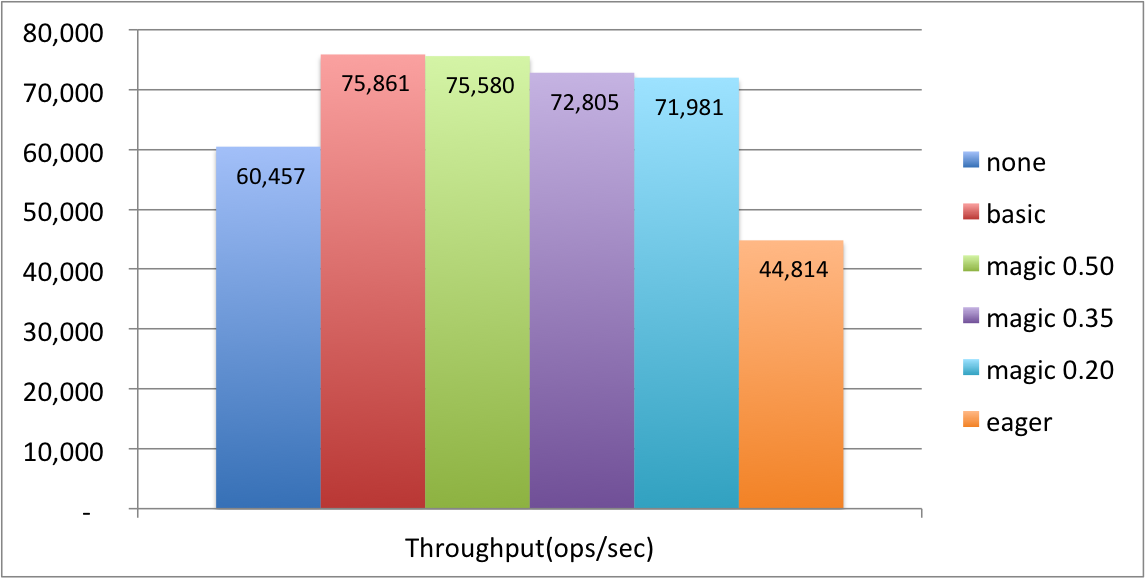
\includegraphics[width=\figw]{Figs/throughput-ssd-uniform.png}
\caption{{\bf  Throughput measured in SSD.} Uniform distribution.
}
\label{fig:throughput-ssd-uniform}
\end{figure}

\begin{figure}[htb]
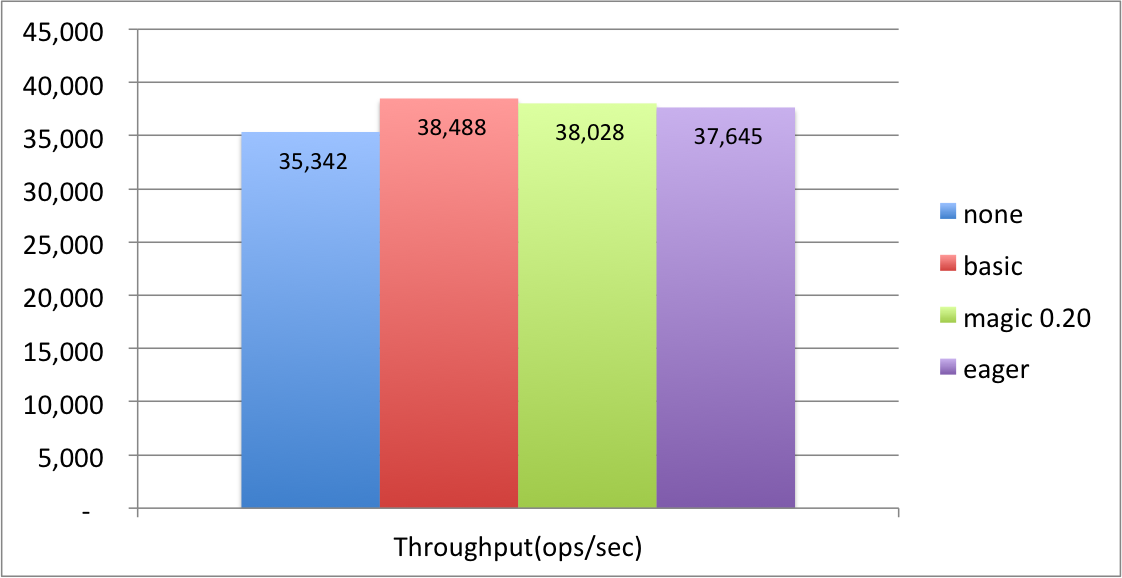
\includegraphics[width=\figw]{Figs/throughput-hdd-uniform.png}
\caption{{\bf  Throughput measured in HDD.} Uniform distribution. 
}
\label{fig:throughput-hdd-uniform}
\end{figure}

\begin{figure}[htb]
%\includegraphics[width=\figw]{Figs/volume-ssd-uniform.png}
\caption{{\bf  Write volume in SSD.} Zipf distribution.
}
\label{fig:volume-ssd-uniform}
\end{figure}

\begin{figure}[htb]
%\includegraphics[width=\figw]{Figs/volume-hdd-uniform.png}
\caption{{\bf  Write volume in HDD.} Zipf distribution.
}
\label{fig:volume-hdd-uniform}
\end{figure}



\paragraph{Mixed workload.}
Each run is comprised of two phases. 
The first phase creates an empty 50 regions table. It then loads the table with 10GB of data by running 100 million update operations chosen uniformly at random, each writing to all columns. 
The second phase measures the performance of a single thread running 150,000 read operation. 
We measure the 50th, 75th, 90th, 95th and 99th percentiles.
An additional YCSB client is used to run background traffic. 
This client utilizes 12 threads to run update operations while we measure the read operations. 
Both reads and background traffic are chosen from a Zipf distribution.
Each such run is repeated three times. 

Figure~\ref{fig:latency-speedup-hdd} depicts the latency speed-up \basic\ and \magic\ achieve over \none.

\begin{figure}[htb]
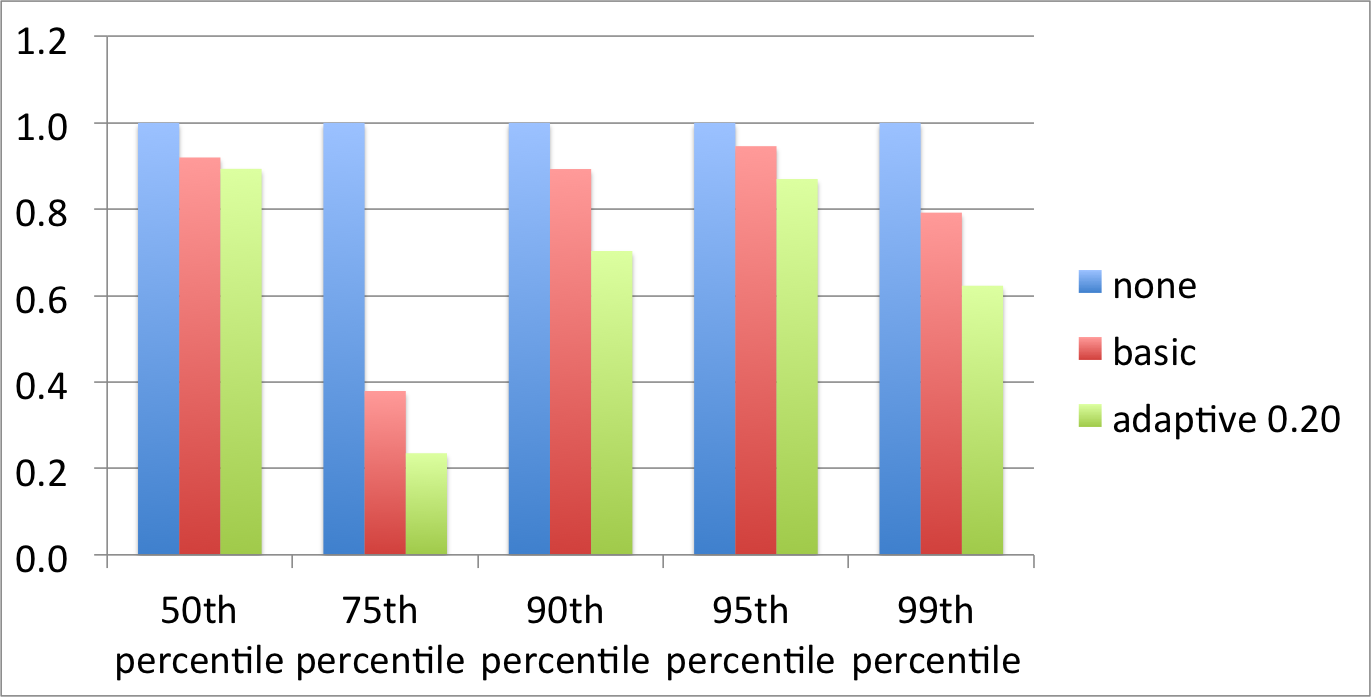
\includegraphics[width=\figw]{Figs/latency-speedup-hdd.png}
\caption{{\bf Latency speed-up in HDD.} 
}
\label{fig:latency-speedup-hdd}
\end{figure}
}

\subsubsection{Parameter Tuning} \label{ssec:tuning}
One of the main sources of memory management overhead is the skiplist data structure used to index the active  memory segment.
Not only  is it bigger in size compared to a flat index, it is also fragmented whereas a static index is stored in a consecutive block of memory. Therefore, flat storage incurs smaller overhead in terms of allocation, GC, and cache misses.
We first tune the size of this data structure.

We evaluate the \basic\ policy with different bounds on the active segment fraction: $A=0.25$, $0.1$, $0.05$, and $0.02$. 
\none\ has no static memory segments, hence its throughput is designated with a single point  $A=1$.
We measure  throughput in a write-only Zipf workload, on SSD,  for the four values of $A$, and with a pipeline size $S=2$.
The throughput of all five runs for each segment size are depicted in  Figure~\ref{fig:dynamic-fraction}. 
The store scales as the active segment memory fraction decreases. 

\begin{figure}[htb]
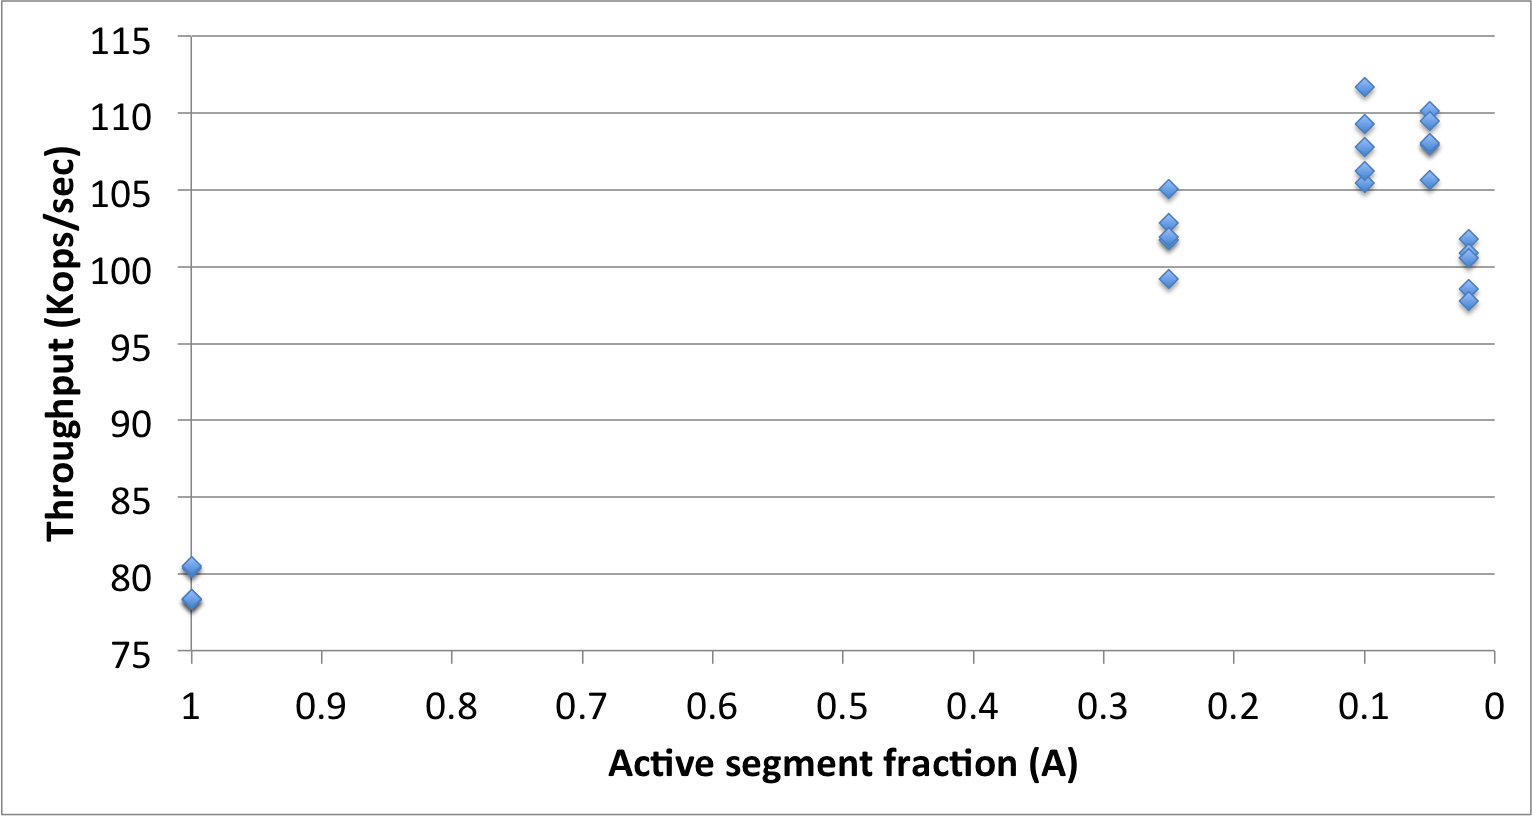
\includegraphics[width=\figw]{Figs/dynamic-fraction-1.png}
\caption{Tuning of the active segment memory fraction, $A$, for the \basic\/ policy, with $S=2$,
Zipf distribution on SSD.  Five experiments are conducted for each $A$. 
The write throughput is higher for small values of $A$.
}
\label{fig:dynamic-fraction}
\end{figure}

The next parameter is the pipeline size.
When $A$ is less than $10\%$, it is clear that merging the active segment into the much bigger static data structure
over and over again can be inefficient, as it creates a new index and releases the old one. 
The alternative is to batch multiple segments in the pipeline before merging into a single segment. 
This throttles the index creation rate. On the flip side, the read API's must scan all the segments, 
which degrades their performance.
%Hence, we run the same experiments as explained above, varying the limit for the size of pipeline.
Figure~\ref{fig:pipeline} depicts the throughput results as a function of the number of segments in the pipeline. 
The peak throughput is achieved with $S=5$ on SSD and $S=4$ and HDD.

\begin{figure*}[tb]

  \centering
  
  \begin{subfigure}[t]{\columnwidth}
      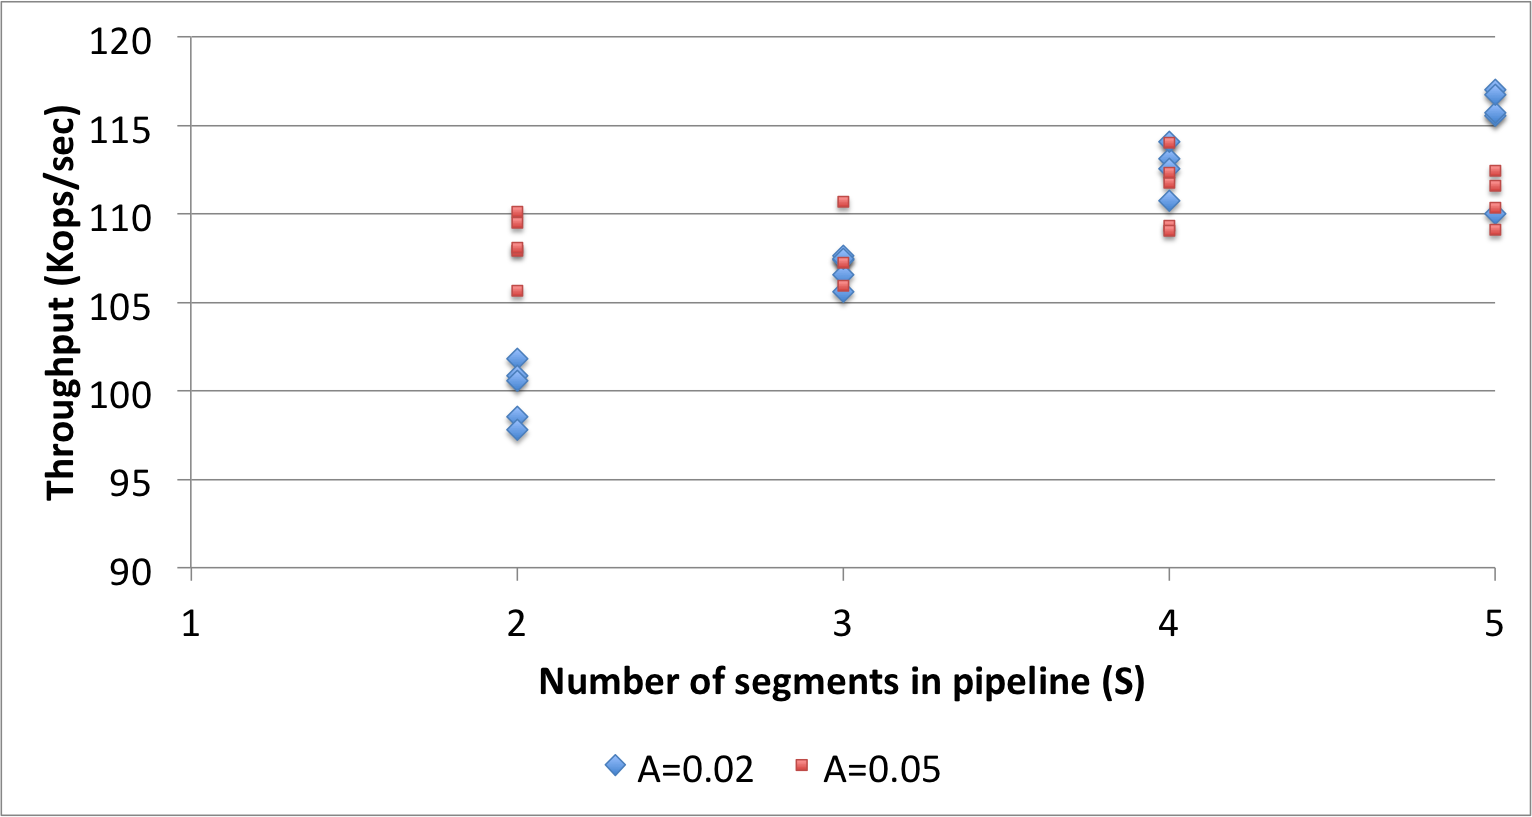
\includegraphics[width=\figw]{Figs/pipeline-1-ssd.png}
      \caption[]{SSD}
    \label{fig:pipeline:ssd}  
  \end{subfigure}   
  \begin{subfigure}[t]{\columnwidth}
      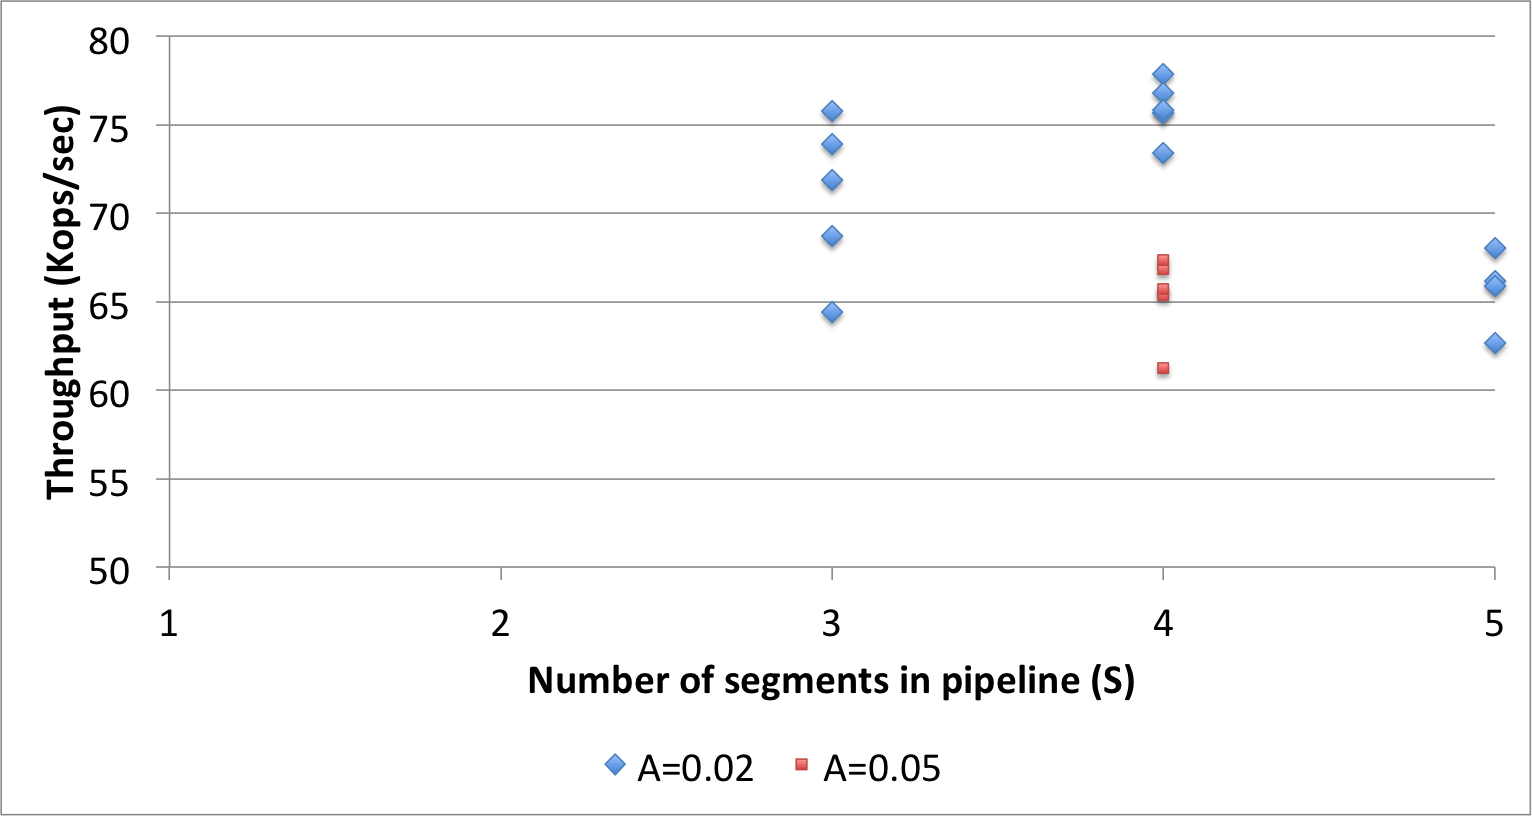
\includegraphics[width=\figw]{Figs/pipeline-1-hdd.png}
      \caption[]{HDD}
    \label{fig:pipeline:hdd}
  \end{subfigure}

\caption{Tuning of the pipeline size bound, $S$, for the \basic\/ policy. Five experiments are conducted for each $S$.} 
\label{fig:pipeline}
\end{figure*}

With the optimal active segment size found for \basic\ ($A=0.02$), \eager\/ performs poorly since compacting the data so frequently is inefficient. 
Figure~\ref{fig:eager-throughput} shows that when the active segment is much bigger ($A=0.25$), \eager\ performs better, and outperforms the 
baseline by $20$\%. We also discovered that the write volume for \eager\ is the roughly the same in these two settings whereas \basic's write volume 
increases with $A$.ß (these results are not shown).  
Since \adp\ is always superior to \eager, we excluded \eager\ from the experiments reported above.  

\begin{figure}[htb]
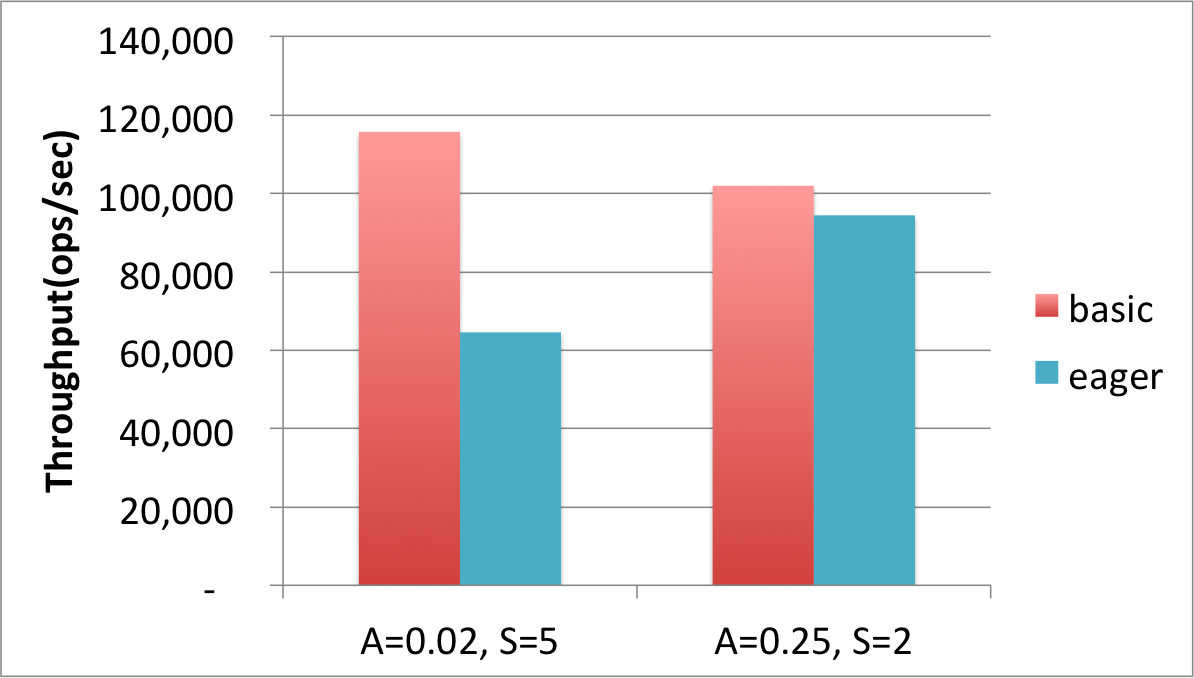
\includegraphics[width=\figw]{Figs/eager-throughput.png}
\caption{Throughput (op/sec): \eager\/ versus \basic\/ in different settings.
}
\label{fig:eager-throughput}
\end{figure}



\remove{
With a different experimental setup the tuning results are different.
For example when running similar workload with 100 regions and 16GB heap per region server we get different results.
\begin{figure}[htb]
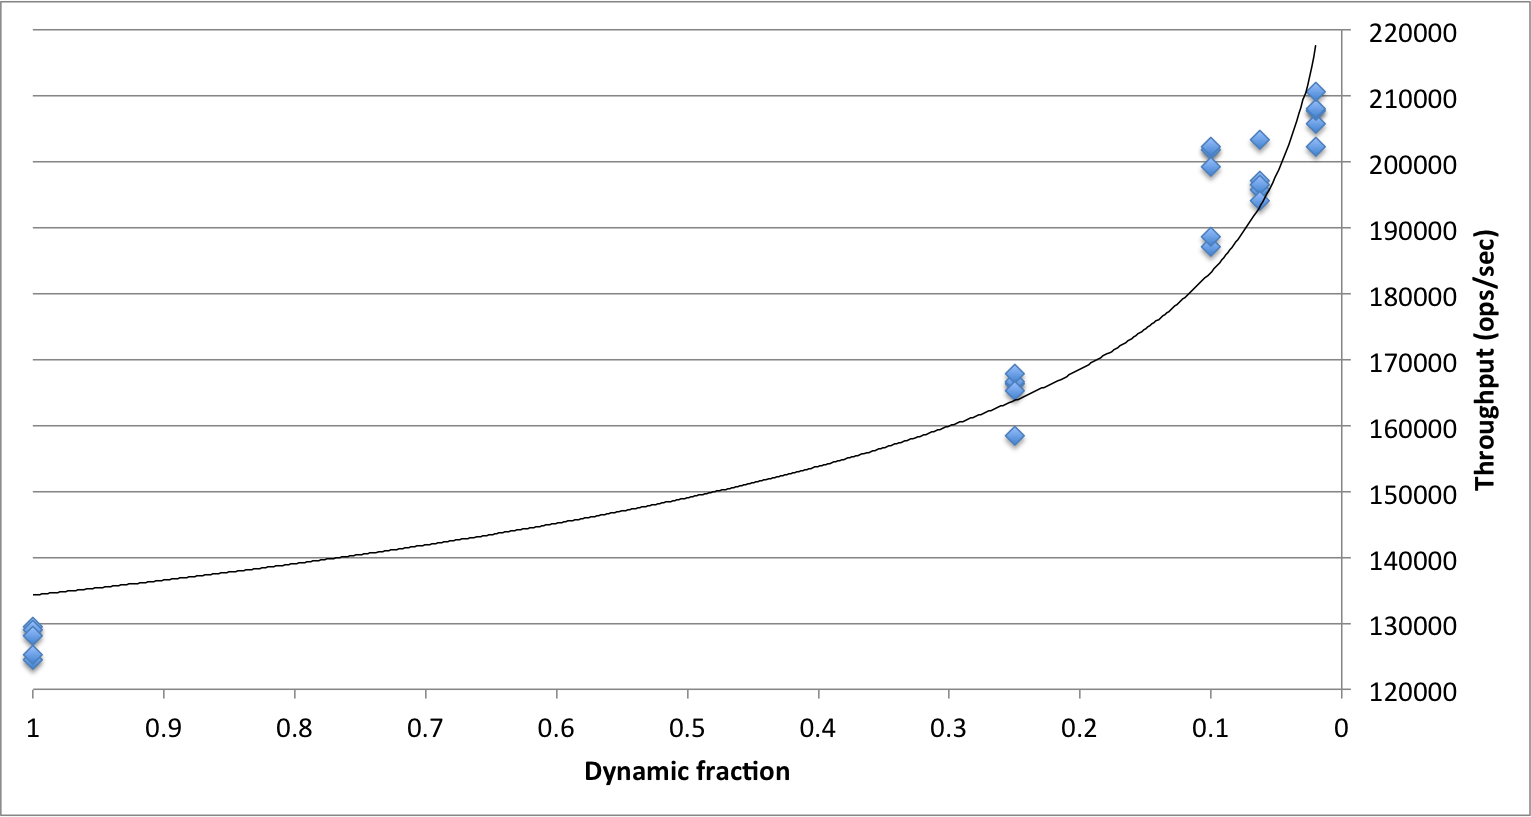
\includegraphics[width=\figw]{Figs/dynamic-fraction-2.png}
\caption{{\bf Dynamic fraction tuning.} 
}
\label{fig:dynamic-fraction-2}
\end{figure}

\begin{figure}[htb]
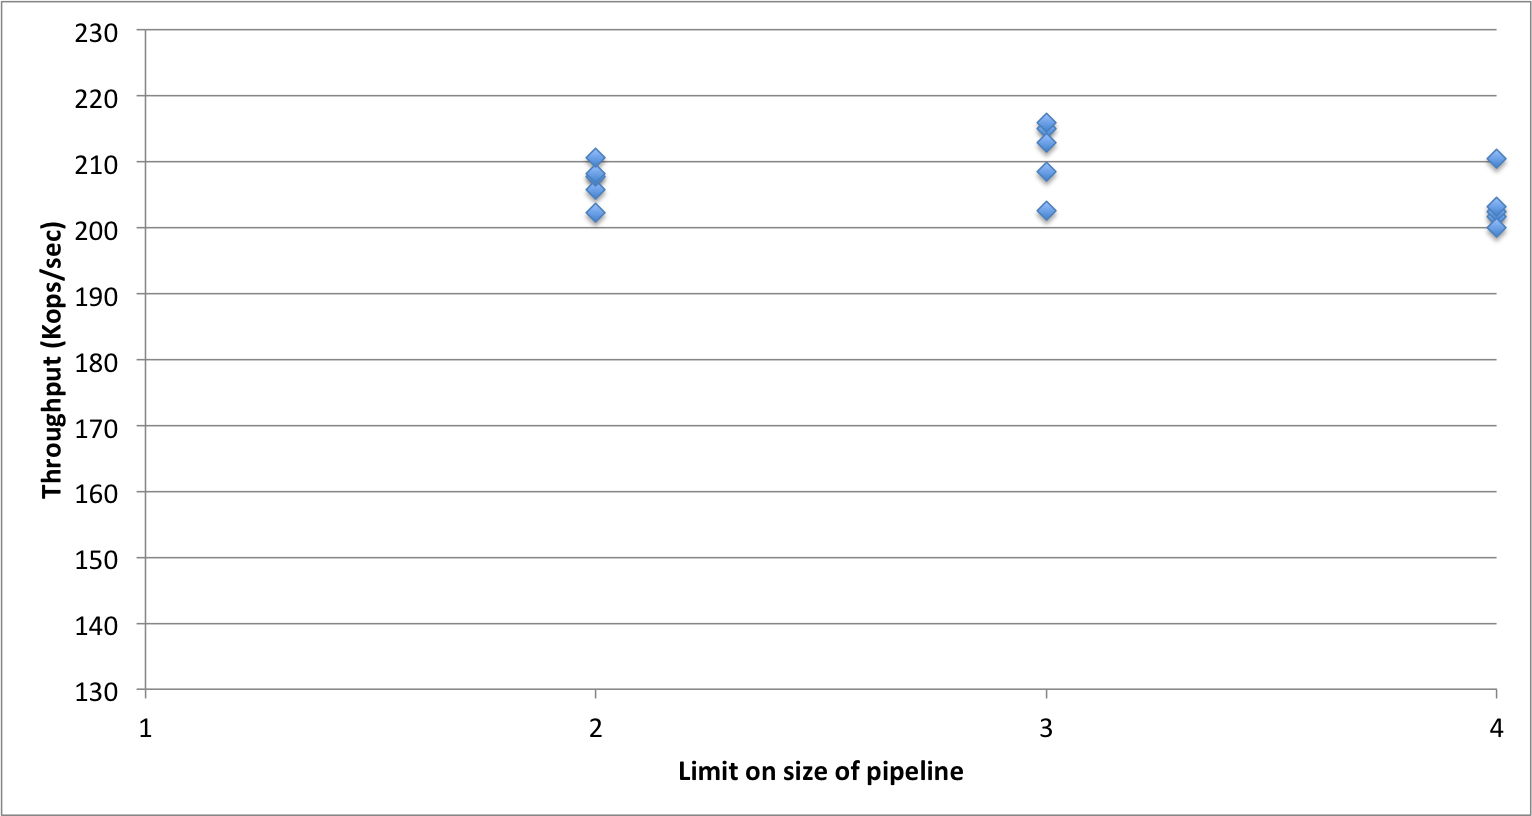
\includegraphics[width=\figw]{Figs/pipeline-2.png}
\caption{{\bf Pipeline size tuning.} 
}
\label{fig:pipeline-2}
\end{figure}


\begin{figure}[htb]
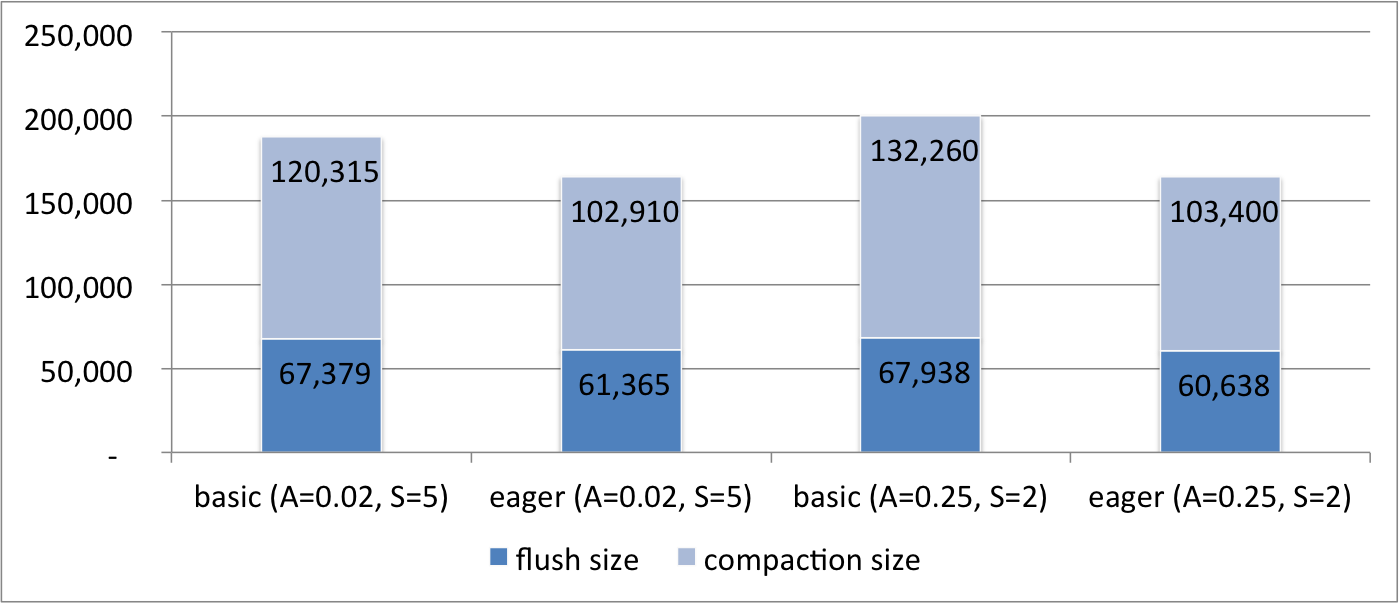
\includegraphics[width=\figw]{Figs/eager-volume.png}
\caption{Write volume: \eager\/ vs \basic\/ in different settings.
}
\label{fig:eager-volume}
\end{figure}
}
